\section{Representation and operator theory}
% Original presentation frame 30
\begin{frame}[t,shrink=5]{Fifteen pairwise marginals preserve useful structure but do not determine the full 6D joint density}
\begin{columns}[T,onlytextwidth]
\begin{column}{0.53\textwidth}
\begin{center}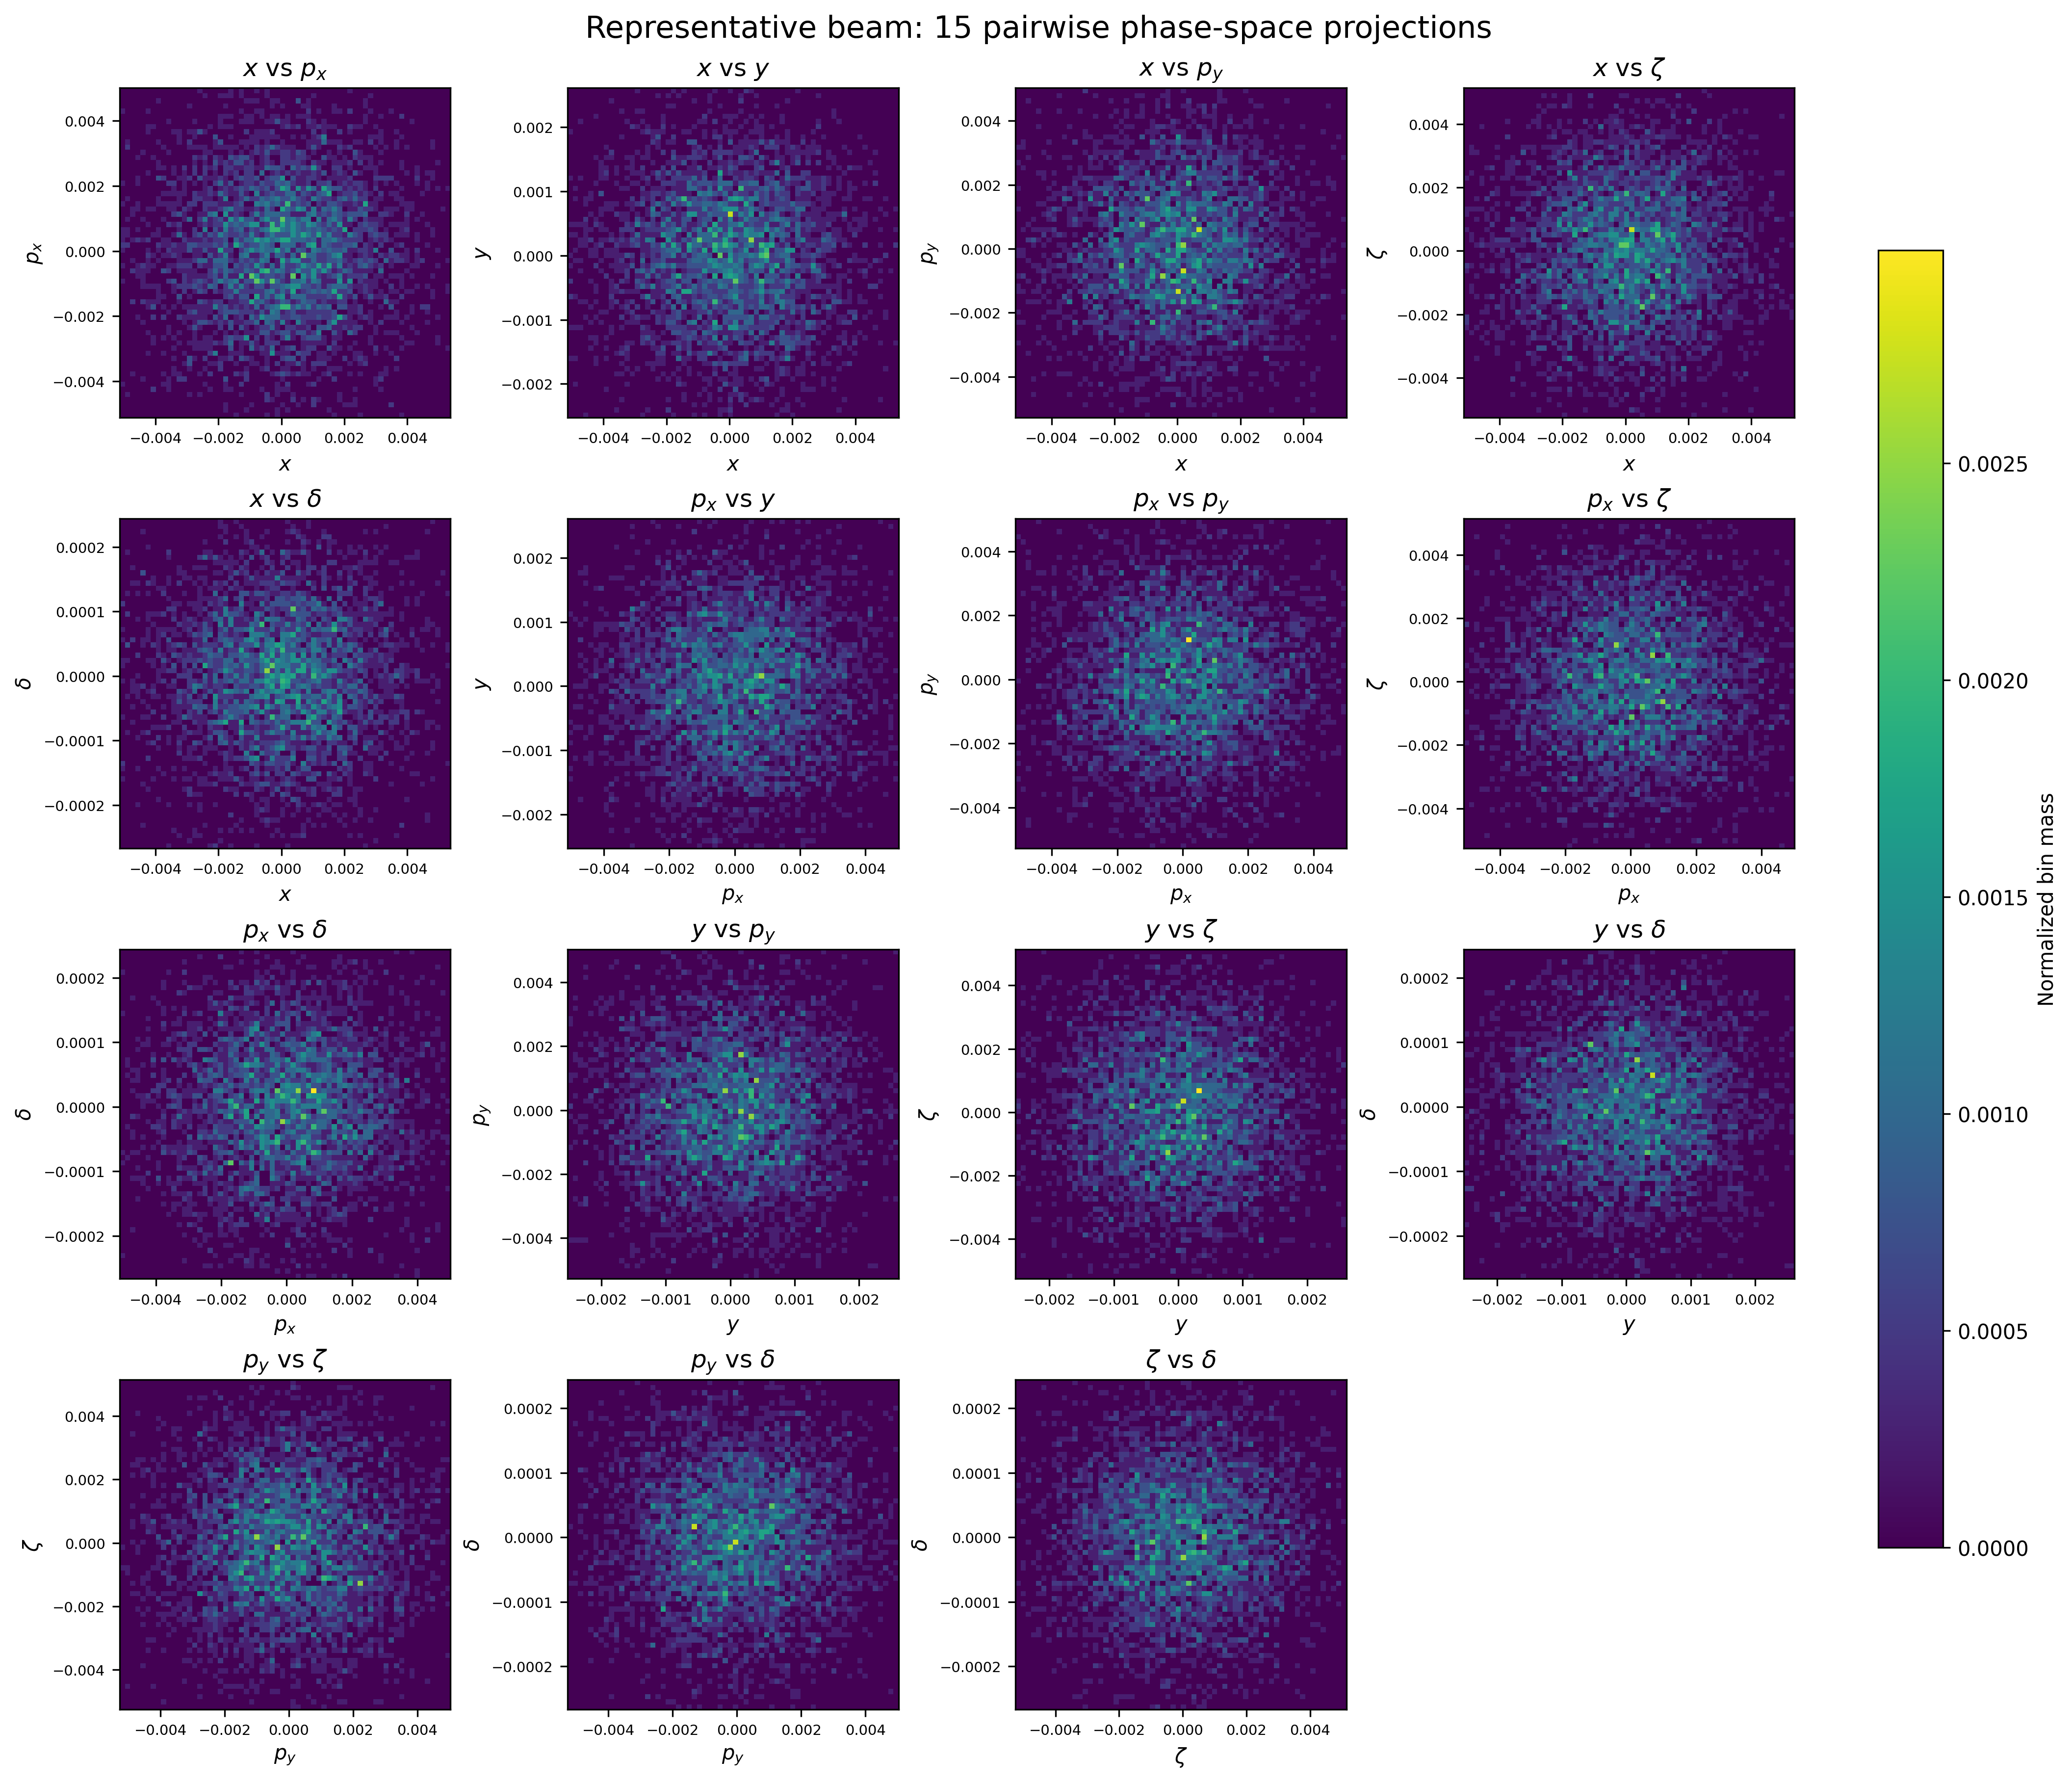
\includegraphics[width=\linewidth,height=53mm,keepaspectratio]{beam_pairwise_phase_space_marginals.png}\end{center}{\scriptsize Fig. 1: fifteen two-dimensional marginals and the separate centroid/RMS vectors.\par}
\end{column}
\begin{column}{0.44999999999999996\textwidth}
\begin{block}{Marginal representation}
\[H(\rho)\in\mathbb R^{15\times64\times64},\quad\sum_{a,b}H_{ij}[a,b]=1.\]
Six centroids and six coordinate-wise RMS spreads restore physical position and scale.
\end{block}
\begin{block}{Uniqueness of the 6D density}
Three- to six-coordinate dependence is absent from the representation. The CVAE error is therefore an error on the fifteen projections, not on an unknown complete 6D density.
\end{block}

\end{column}
\end{columns}

\sources{\parencite{hoover2024tomography}.}

\end{frame}

% Original presentation frame 31
\begin{frame}[t,shrink=5]{The latent coordinates show no pervasive linear alignment with the 12 explicit beam statistics}
\begin{columns}[T,onlytextwidth]
\begin{column}{0.69\textwidth}
\begin{center}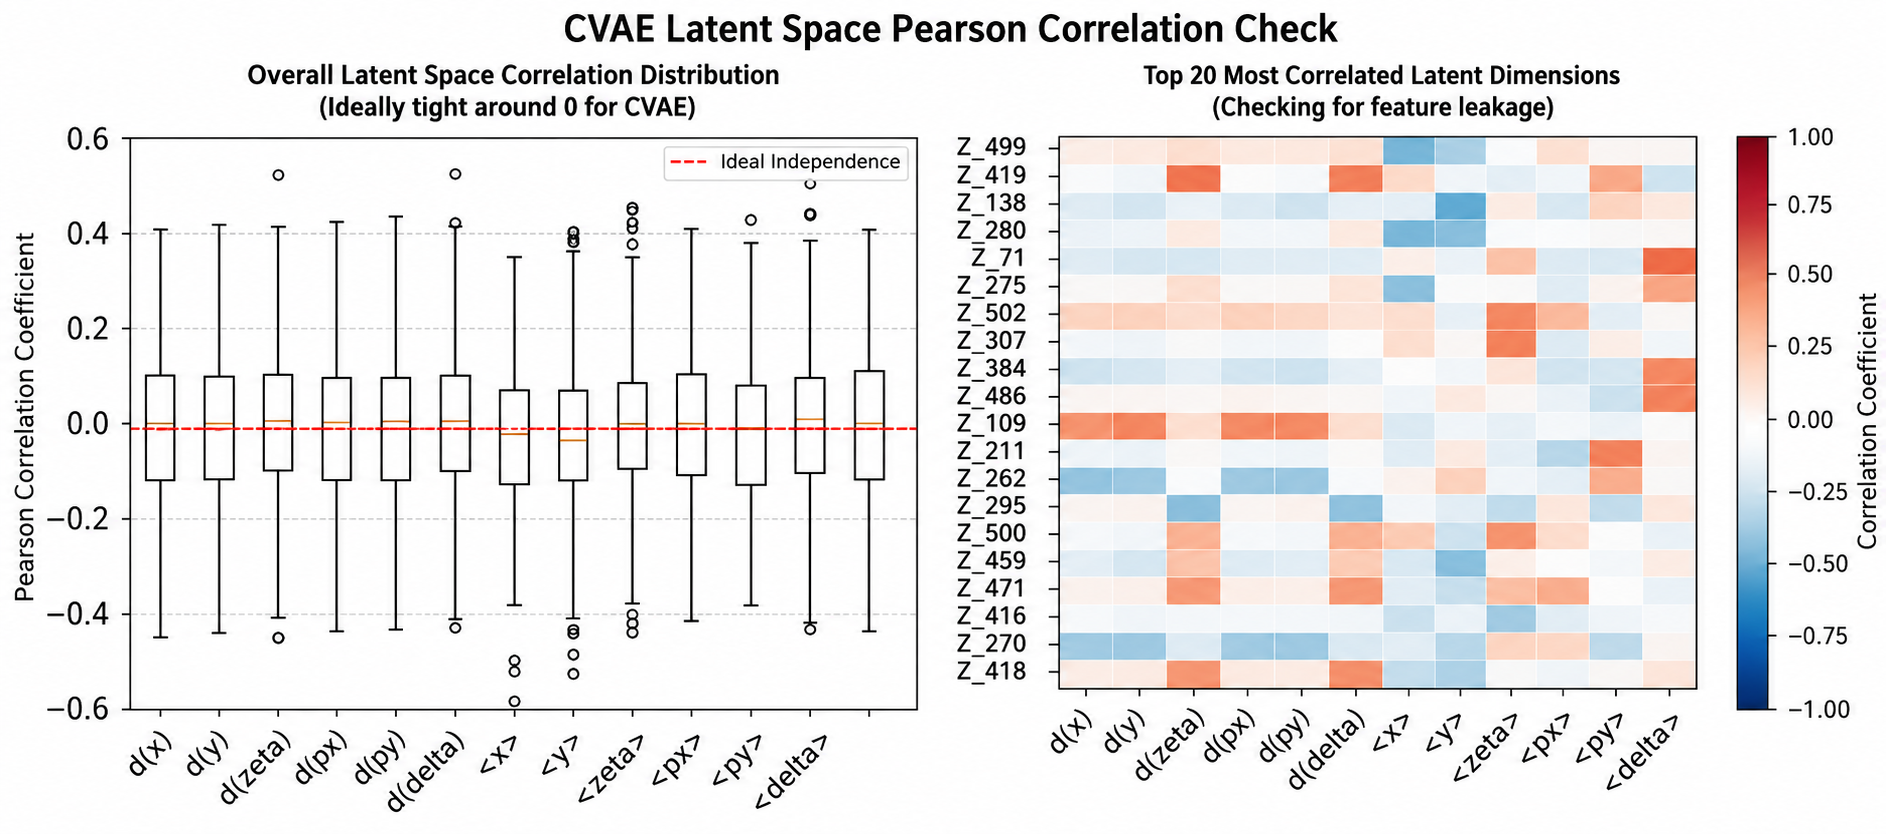
\includegraphics[width=\linewidth]{latent_physical_correlations.png}\end{center}
\end{column}
\begin{column}{0.29000000000000004\textwidth}
\begin{block}{Test}
$512\times12=6144$ Pearson coefficients on $N_{\rm val}=51$ samples.
\end{block}
\begin{block}{Observed}
Mean $|r|=0.1161$, median $|r|=0.1006$, maximum $|r|=0.5333$.
\end{block}
\begin{block}{In summary}
Evidence against systematic linear leakage, not proof of independence or nonlinear disentanglement.
\end{block}

\end{column}
\end{columns}

\sources{CVAE formulation: \parencite{kingma2014vae,sohn2015cvae}.}

\end{frame}

% Original presentation frame 32
\begin{frame}[t,shrink=5]{Windowed attention is a GNO with a normalized exponential kernel}
Common causal support: $\mathcal N_i\equiv\mathcal N_w^{-}(i)=\{j:\max(1,i-w+1)\le j\le i\}$. Score: $s_{ij}^{(\ell)}=q_i^{(\ell)\top}k_j^{(\ell)}/\sqrt{d_k}$.\begin{columns}[T,onlytextwidth]
\begin{column}{0.49\textwidth}
\begin{block}{1. Write local attention as a graph kernel}
\[\alpha_{ij}^{(\ell,w)}=\mathbf1_{j\in\mathcal N_i}\frac{\exp(s_{ij}^{(\ell)})}{\sum_{r\in\mathcal N_i}\exp(s_{ir}^{(\ell)})}.\]
\[K_{\rm TF,ij}^{(\ell)}=\alpha_{ij}^{(\ell,w)}W_O^{(\ell)}W_V^{(\ell)},\]
\[\widetilde h_{i,\rm TF}^{(\ell+1)}=h_i^{(\ell)}+\sum_{j\in\mathcal N_i}K_{\rm TF,ij}^{(\ell)}h_j^{(\ell)}.\]
\end{block}

\end{column}
\begin{column}{0.49\textwidth}
\begin{block}{2. Select the corresponding GNO objects}
\[\widetilde h_{i,\rm GNO}^{(\ell+1)}=h_i^{(\ell)}+\sum_{j\in\mathcal N_{\rm GNO}(i)}\omega_{ij}K_{\theta,ij}^{(\ell)}h_j^{(\ell)}.\]
\[\mathcal N_{\rm GNO}(i)=\mathcal N_i,\quad\omega_{ij}=1,\]
\[K_{\theta,ij}^{(\ell)}=K_{\rm TF,ij}^{(\ell)}=\alpha_{ij}^{(\ell,w)}W_O^{(\ell)}W_V^{(\ell)}.\]
\end{block}

\end{column}
\end{columns}
\begin{alertblock}{Exact consequence after substitution}
\[\widetilde h_{i,\rm GNO}^{(\ell+1)}=h_i^{(\ell)}+\sum_{j\in\mathcal N_i}K_{\rm TF,ij}^{(\ell)}h_j^{(\ell)}=\widetilde h_{i,\rm TF}^{(\ell+1)}.\]Exact for one head; multi-head \ensuremath{=} kernel sum, while a learned GNO need not obey the softmax form.
\end{alertblock}

\sources{\parencite{li2020graph,vaswani2017attention}.}

\end{frame}

% Original presentation frame 33
\begin{frame}[t,shrink=5]{The single-seed window sweep has a non-monotonic minimum at intermediate support}
\begin{columns}[T,onlytextwidth]
\begin{column}{0.6\textwidth}
\begin{center}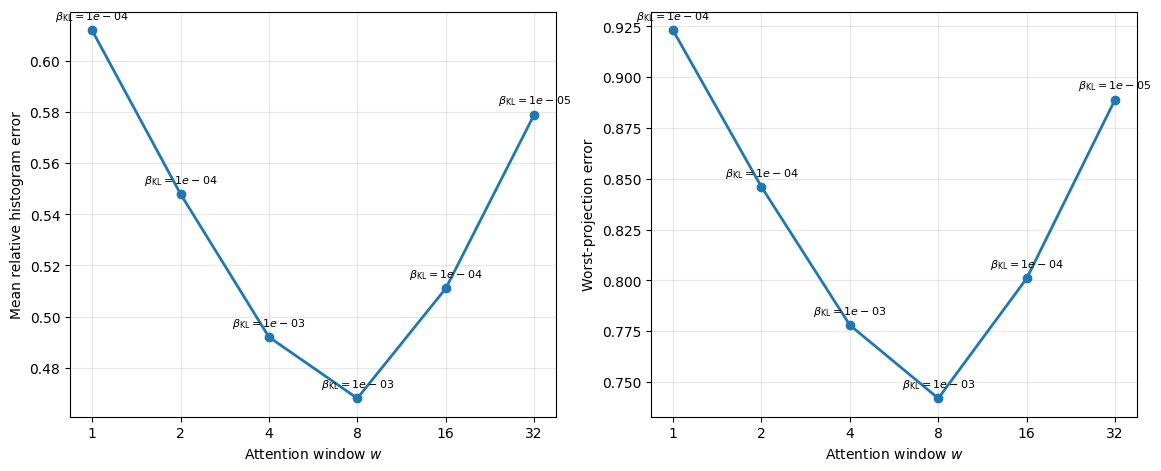
\includegraphics[width=\linewidth]{transformer_window_study.png}\end{center}\begin{center}\begin{adjustbox}{max width=\linewidth}
\begin{tabular}{rrrrr}\toprule $w$ & $\beta_{\rm KL}$ & Mean error & Worst & Mean KL\\\midrule
1 & $10^{-4}$ & .612 & .923 & .418\\2 & $10^{-4}$ & .548 & .846 & .356\\4 & $10^{-3}$ & .492 & .778 & .238\\8 & $10^{-3}$ & .468 & .742 & .211\\16 & $10^{-4}$ & .511 & .801 & .304\\32 & $10^{-5}$ & .579 & .889 & .447\\\bottomrule\end{tabular}
\end{adjustbox}\end{center}
\end{column}
\begin{column}{0.38\textwidth}
\begin{block}{Observed trend}
\begin{itemize}
\item Very narrow support omits multi-element context,
\item Intermediate support gives the lowest validation error in this run,
\item Broad support progressively recovers dense upstream mixing.
\end{itemize}
\end{block}

\end{column}
\end{columns}

\sources{Attention architecture: \parencite{vaswani2017attention}.}

\end{frame}

% Original presentation frame 34
\begin{frame}[t,shrink=5]{The reported variance measures sensitivity to CVAE posterior sampling at fixed input and fixed weights}
\begin{block}{Random quantity and Monte-Carlo estimator}
\[z_0^{(r)}=\mu_\phi(X_0,c)+\sigma_\phi(X_0,c)\odot\epsilon^{(r)},\quad\epsilon^{(r)}\sim\mathcal N(0,I),\]
\[Y^{(r)}=\mathcal D_\psi\left(\mathcal T_\theta^N(z_0^{(r)},\{h_i\},\mu),c_N\right),\]
\[\widehat{\operatorname{Var}}_z[Y\mid X_0,c,\mu,\theta]=\frac1R\sum_{r=1}^{R}\left(Y^{(r)}-\overline Y\right)^2.\]
$Y$ may be one histogram bin, physical density bin, centroid or RMS spread.
\end{block}
\begin{columns}[T,onlytextwidth]
\begin{column}{0.49\textwidth}
\begin{block}{Fixed inputs and weights}
Input beam, conditioning variables, machine parameters, lattice tokens and trained weights $\theta$.
\end{block}
\begin{block}{Measured statistics}
Variability caused by the stochastic conditional latent state of this one trained CVAE--GNO model.
\end{block}

\end{column}
\begin{column}{0.49\textwidth}
\begin{alertblock}{Not included in total predictive uncertainty}
Weight/parameter uncertainty, finite-data effects, architecture and model-form discrepancy, simulator discrepancy, measurement noise and OOD error.
\end{alertblock}

\end{column}
\end{columns}

\sources{Variational posterior: \parencite{kingma2014vae,sohn2015cvae}.}

\end{frame}

% Original presentation frame 35
\begin{frame}[t,shrink=5]{Latent sampling does not cover the dominant energy-spread error of the physical-statistics head}
\begin{columns}[T,onlytextwidth]
\begin{column}{0.6\textwidth}
\begin{center}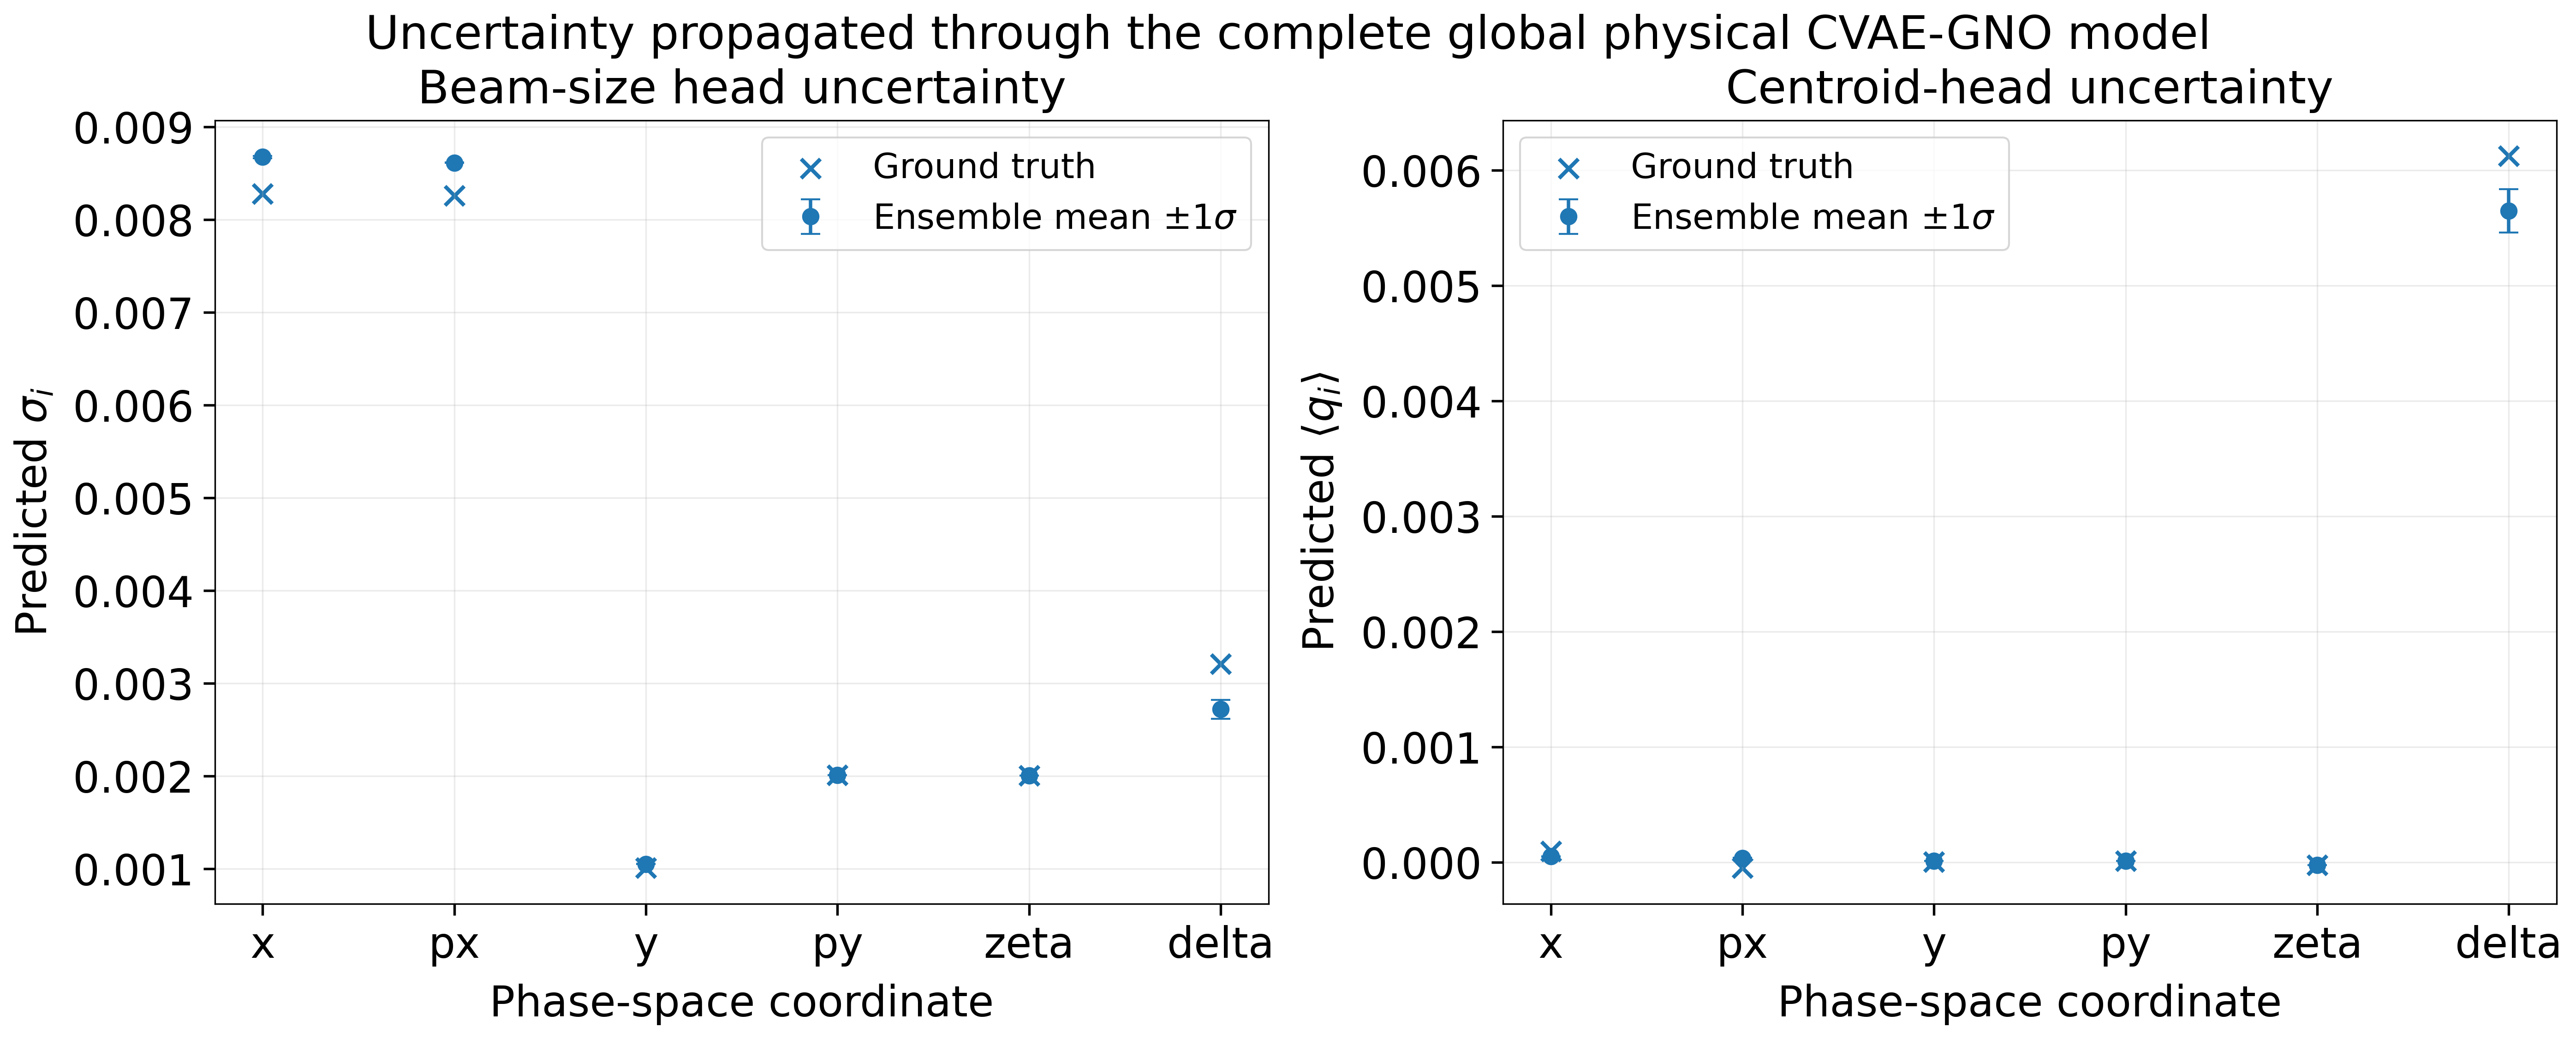
\includegraphics[width=\linewidth]{latent_variability_rms_and_centroids.png}\end{center}{\scriptsize Ensemble mean $\pm$ one latent-sampling standard deviation and reference values for six RMS spreads and centroids.\par}
\end{column}
\begin{column}{0.38\textwidth}
\begin{block}{Dimensionless diagnostics}
\[e_{\sigma,d}=\frac{\overline\sigma_d-\sigma_d^{\rm true}}{\sigma_d^{\rm true}},\quad b_{m,d}=\frac{\overline m_d-m_d^{\rm true}}{\sigma_d^{\rm true}}.\]
\end{block}
\begin{block}{Selected sample}
Transverse and longitudinal-position statistics are mostly within a few percent of the relevant beam scale. For $\delta$, the predicted spread is only $11.8\%$ of the reference value, while latent-sampling variability is about $0.026\%$ of that reference spread.
\end{block}

\end{column}
\end{columns}

\end{frame}

